\documentclass[a4paper, 12pt]{article} % report, book, letter
\usepackage{amsmath}
\usepackage{amsthm}
\usepackage{tikz}
\usepackage{pgfplots}
\usepackage{circuitikz}
\usetikzlibrary{shapes.geometric, arrows}
\usetikzlibrary{mindmap}

\theoremstyle{plain} % definition, remark
\newtheorem{teorema}{Teorema}
\newtheorem{corollario}{Corollario}[teorema]
\newtheorem{lemma}{Lemma}[teorema]

\begin{document}
\section{Formule matematiche}
Esempio: $a^2 + b^2 = c^2$. \\
Equazione:
\begin{equation} % numerato
    a^2 + b^2 = c^2
\end{equation}
\begin{equation*} % non numerato amsmath!
    a^2 + b^2 = c^2
\end{equation*}
\begin{equation}
    \lim_{n \to \infty} \sum_{k=1}^n \frac{1}{k^2} = \frac{\pi ^2}{6}
\end{equation}
\begin{equation}
    \forall x \in \mathbf{R}: x^2 \geq 0
\end{equation} % \quad o \qquad per extra spazio
\begin{equation}
    \alpha, \omega, \xi, \delta, \Delta, \pi, \mu, \psi
\end{equation}
\begin{equation}
    e^x \cdot e^y = e^{x+y}
\end{equation}
\begin{equation}
    n! = n\cdot (n-1) \cdots 2 \cdot 1
\end{equation}
\begin{equation}
    \nabla^2 = \frac{\partial^2}{\partial x^2} + \frac{\partial^2}{\partial y^2} + \frac{\partial^2}{\partial z^2}
\end{equation}
\begin{equation}
    \int_0^{2\pi} \sin x \cos x \,dx = 0
\end{equation}
\begin{equation} % integrale fisico
    \oint_{\gamma} f(\vec{s}\,) \,d\vec{s}
\end{equation}
\begin{equation}
    (\frac{1}{1+\frac{1}{x^2}})^3
\end{equation}
\begin{equation}
    \left( \frac{1}{1+\frac{1}{x^2}} \right) ^3
\end{equation}

% matrici
\begin{equation}
    \mathbf{X} = \left( 
    \begin{array}{ccc}
    x_1 & x_2 & \ldots \\
    x_3 & x_4 & \ldots \\
    \vdots & \vdots & \ddots 
    \end{array} \right)
\end{equation}

% definizione modulo
\begin{equation}
    |x| = \left\{
    \begin{array}{rl}
    -x & \text{if } x < 0, \\
    0 & \text{if } x = 0, \\
    x & \text{if } x > 0.
    \end{array} \right.
\end{equation}

% teoremi, lemmi e dimostrazioni
% \usepackage{amsthm}
\begin{teorema}
    Se f è derivabile $\forall x \in \mathbf{R}$, allora f è continua su $\mathbf{R}$.
\end{teorema}

\begin{teorema}[di Pitagora]
\label{pitagora}
\begin{equation*}
    a^2 + b^2 = c^2 
\end{equation*}
\end{teorema}
\begin{proof}
    Algebretta lasciata al lettore.
\end{proof}

\begin{corollario}
    Come conseguenza del teorema \ref{pitagora}, non esiste un triangolo rettangolo di lati 3cm, 4cm e 6cm.
\end{corollario}

\begin{lemma}
    Come conseguenza del teorema \ref{pitagora}, la lunghezza del lato lungo di un triangolo è inferiore alla somma delle lunghezze dei due lati corti.
\end{lemma}

% per una lista molto completa di simboli matematici che potrebbero tornare utili fare riferimento a pagina 65 della guida lasciata sul sito. 

\newpage
\section{Disegni in \LaTeX}
% \usepackage{tikz}

\begin{tikzpicture}[scale=1]
\draw[red] (0,0) -- (4,0);

\draw (0,1) -- (4,1) -- (4,5) -- (0,5) -- (0,1);

\draw (0,6) rectangle (4,10);

\draw (2,-5) circle (3cm);

\draw[blue,thick,dashed] (2,-5) ellipse (5cm and 1cm);

\filldraw[fill=yellow, draw=black] (2,-5) circle (0.8cm);
\end{tikzpicture}

\newpage
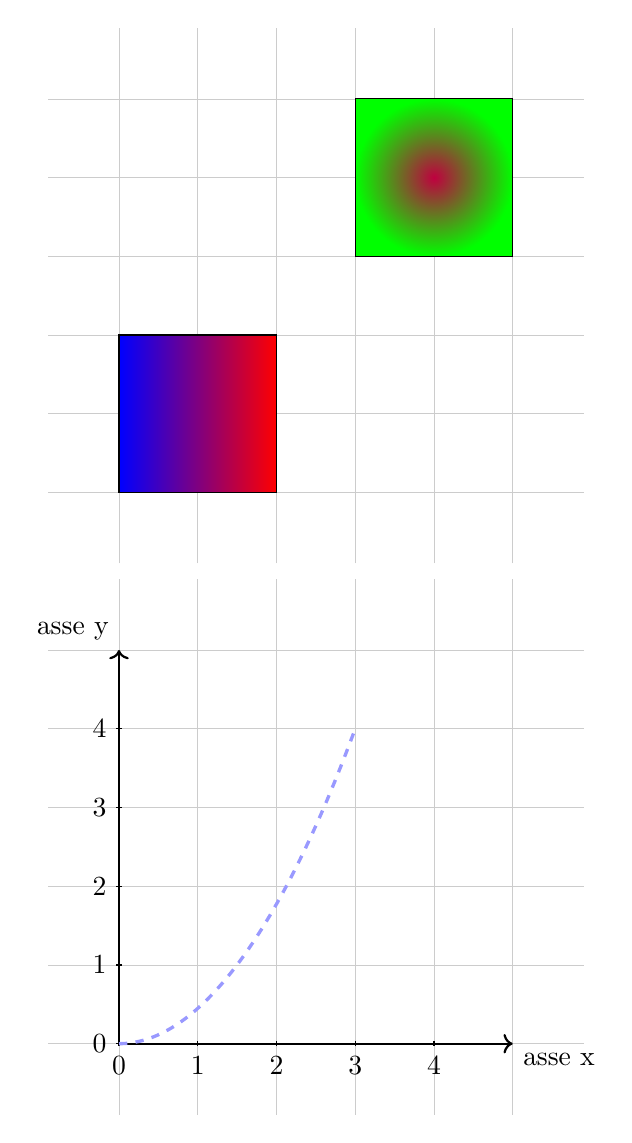
\begin{tikzpicture}[scale=1]
%\draw[step=1cm,gray,very thin] (-1,-1) grid (6,6);

\draw[step=1cm,gray!40!white,very thin] (-0.9,-0.9) grid (5.9,5.9);

\shade[left color=blue,right color=red,draw=black] (0,0) rectangle (2,2);

\shade[inner color=purple,outer color=green,draw=black] (3,3) rectangle (5,5);

\draw[step=1cm,gray!40!white,very thin] (-0.9,-7.9) grid (5.9,-1.1);

\draw[thick,->] (0,-7) -- (5,-7) node[anchor=north west] {asse x};
\draw[thick,->] (0,-7) -- (0,-2) node[anchor=south east] {asse y};

\foreach \x in {0,1,2,3,4}
   \draw (\x cm,-7cm+1pt) -- (\x cm,-7cm-1pt) node[anchor=north] {$\x$};
\foreach \y in {0,1,2,3,4}
    \draw (1pt,-7cm+\y cm) -- (-1pt,-7cm+\y cm) node[anchor=east] {$\y$};

\draw[blue!40!white,very thick,dashed] (0,-7) parabola (3,-3);
\end{tikzpicture}

% GeoGebra supporta la funzione per generare il codice TikZ di un dato grafico!

\newpage
% \usepackage{pgfplots}
\subsection{Grafici}
\begin{center}
\begin{tikzpicture}
\begin{axis}
\addplot[color=green]{exp(x)};
\end{axis}
\end{tikzpicture}
\end{center}

% \usepackage{circuitikz}
\subsection{Circuiti}
\begin{center}
\begin{circuitikz} 
\draw (0,0) to[battery] (0,4)
  to[ammeter] (4,4) 
  to[R] (4,0)
  to[C] (0,0)
  (0.5,0) -- (0.5,-2)
  to[voltmeter] (3.5,-2) -- (3.5,0);
\end{circuitikz}    
\end{center}

\subsection{Flowcharts}

%\usetikzlibrary{shapes.geometric, arrows}

% stile (più dettagli su overleaf)
\tikzstyle{startstop} = [rectangle, rounded corners, minimum width=3cm, minimum height=1cm,text centered, draw=black, fill=red!25!white]
\tikzstyle{io} = [trapezium, trapezium left angle=60, trapezium right angle=120, minimum width=3cm, minimum height=1cm, text centered, draw=black, fill=blue!30!white]
\tikzstyle{process} = [rectangle, minimum width=3cm, minimum height=1cm, text centered, draw=black, fill=orange!30]
\tikzstyle{decision} = [diamond, minimum width=3cm, minimum height=1cm, text centered, draw=black, fill=green!30!white]
\tikzstyle{arrow} = [thick,->]

\begin{center}
\begin{tikzpicture}[node distance=2cm]
\node (start) [startstop] {Start};

\node (in1) [io, below of=start] {Input};

\node (pro1) [process, below of=in1] {Process};

\node (dec1) [decision, right of=pro1, xshift=2cm] {Decision};

\draw [arrow] (start) -- (in1);
\draw [arrow] (in1) -- (pro1);
\draw [arrow] (pro1) -- (dec1);
\end{tikzpicture}
\end{center}

\subsection{Mind maps}
\begin{center}
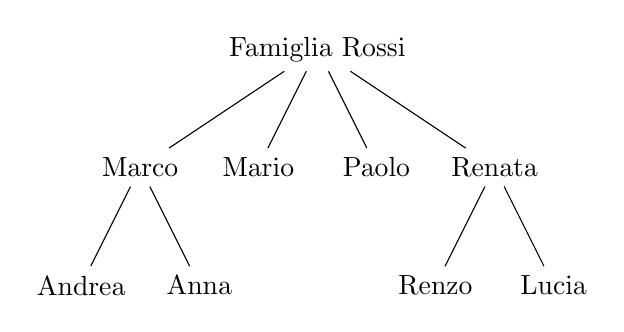
\begin{tikzpicture}

\node{Famiglia Rossi}
	child { node {Marco}
                child { node {Andrea}}
                child { node {Anna}}}
	child { node {Mario}}
	child { node {Paolo}}
	child { node {Renata}
                child { node {Renzo}}
                child { node {Lucia}}}
;
\end{tikzpicture}
\end{center}

\newpage

%\usetikzlibrary{mindmap}
\begin{center}
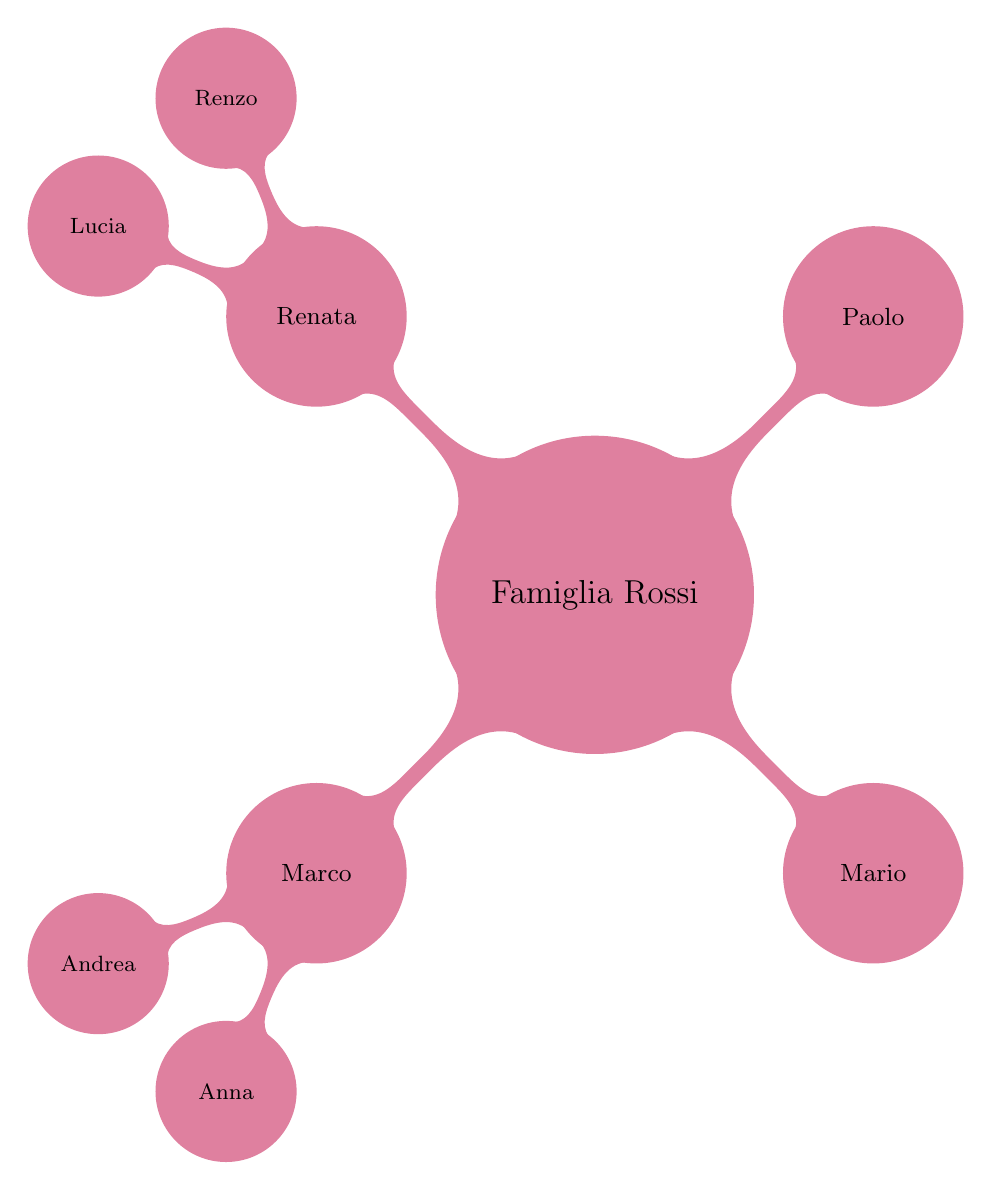
\begin{tikzpicture}[mindmap, grow cyclic, every node/.style=concept, concept color=purple!50!white, 
	level 1/.append style={level distance=5cm,sibling angle=90},
	level 2/.append style={level distance=3cm,sibling angle=45},]
\node{Famiglia Rossi}
	child { node {Marco}
                child { node {Andrea}}
                child { node {Anna}}}
	child { node {Mario}}
	child { node {Paolo}}
	child { node {Renata}
                child { node {Renzo}}
                child { node {Lucia}}}
;
\end{tikzpicture}
\end{center}

\end{document}
